\chapter{Introduction}
\bigskip

\begin{flushright}{\slshape
	It is still an unending source of surprise for me to see \\
	how a few scribbles on a blackboard or on a sheet of paper\\
	could change the course of human affairs.} \\ \medskip
    --- Stanislaw Ulam
\end{flushright}


\noindent If anything good can ever be said about the second world war, it might be this: the war effort sparked a massive number of scientific fields.

\begin{figure}[!p]
\centering

\subfloat[]{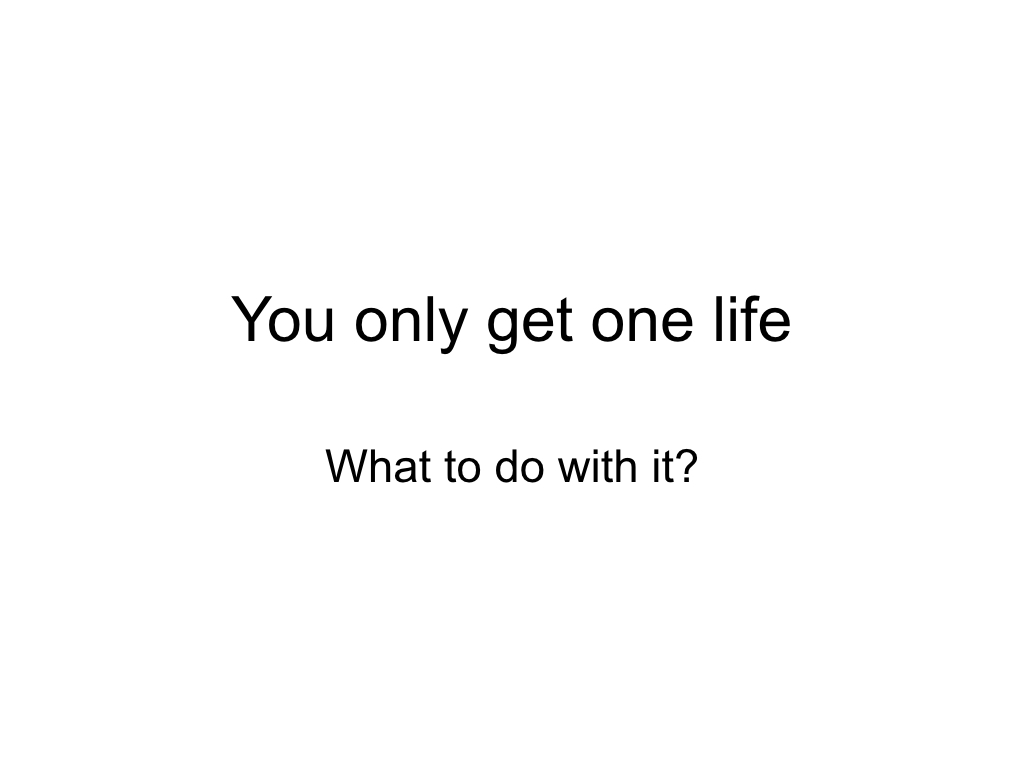
\includegraphics[width=0.5\textwidth]{images02/new-images/Only-one-life077.jpeg}}
\subfloat[]{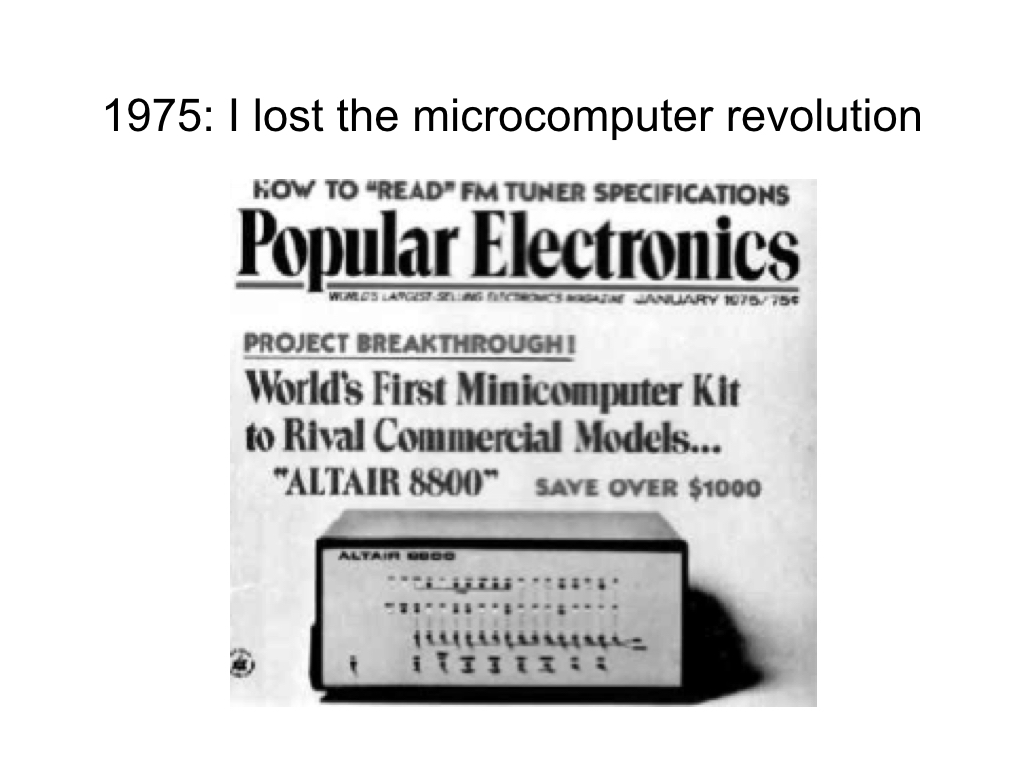
\includegraphics[width=0.5\textwidth]{images02/new-images/Only-one-life078.jpeg}}

\subfloat[]{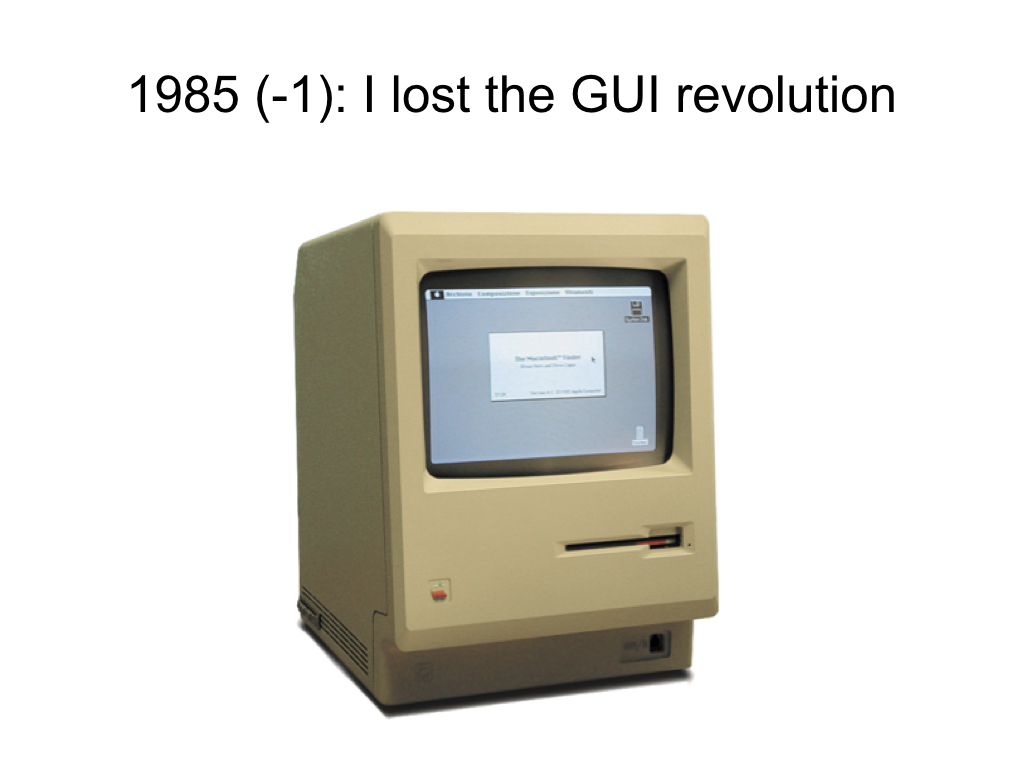
\includegraphics[width=0.5\textwidth]{images02/new-images/Only-one-life079.jpeg}}
\subfloat[]{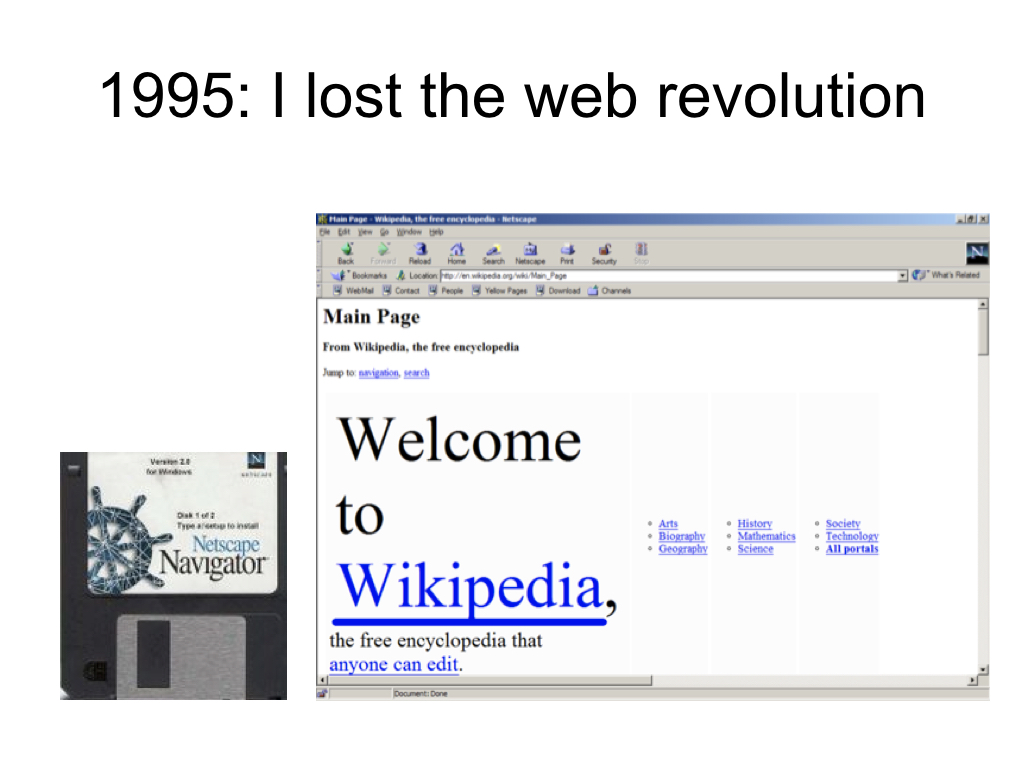
\includegraphics[width=0.5\textwidth]{images02/new-images/Only-one-life080.jpeg}}

\subfloat[]{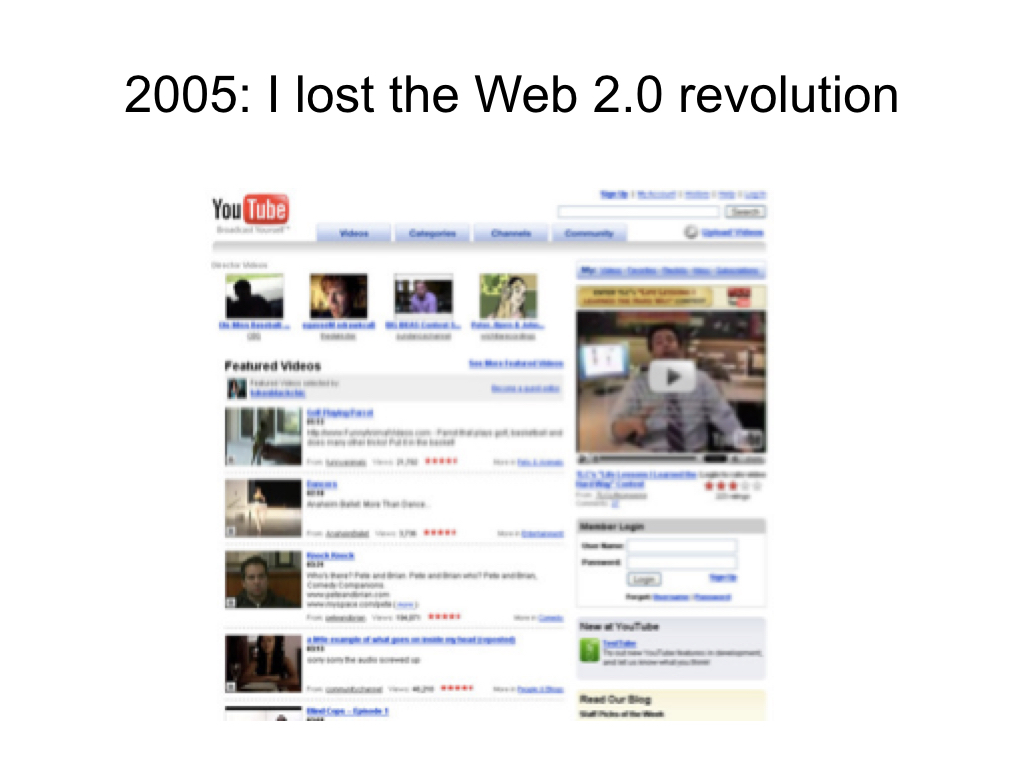
\includegraphics[width=0.5\textwidth]{images02/new-images/Only-one-life081.jpeg}}
\subfloat[]{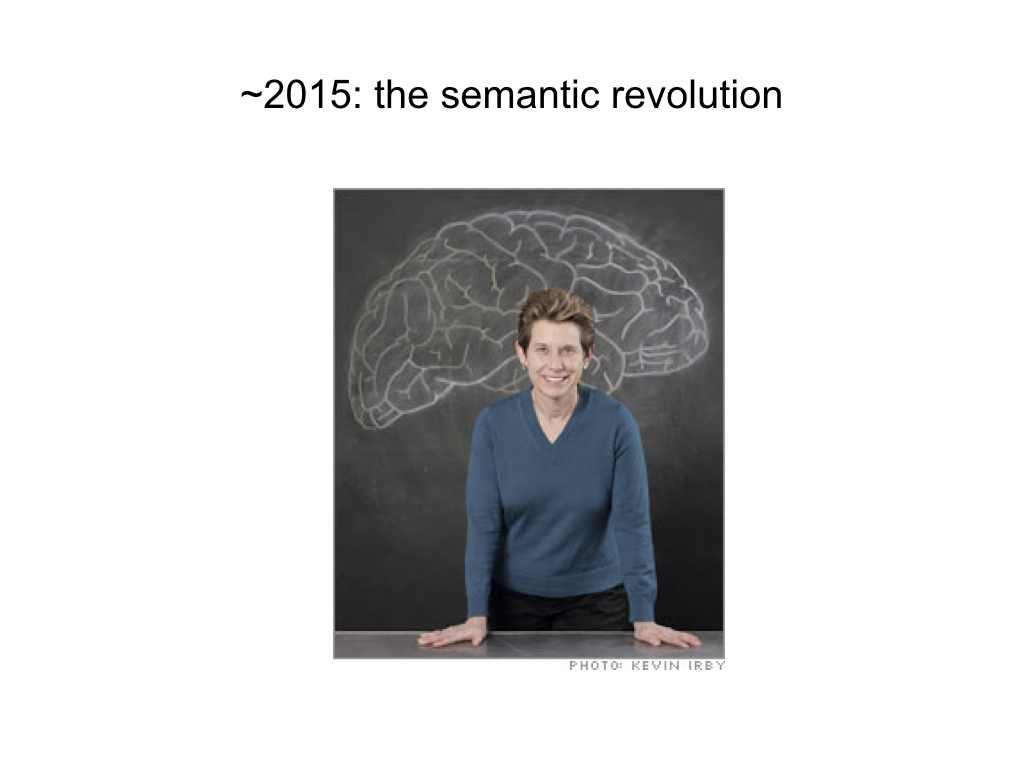
\includegraphics[width=0.5\textwidth]{images02/new-images/Only-one-life082.jpeg}}

\caption{Slides from an old Linhares' class; a viewpoint that has influenced the choice of topics found in this thesis.   In the history of computing business, the most interesting level of analysis seems to be that of the \emph{platform}.  It is where things can get built on top of, and communities emerge, and standards fight against each other, and fortunes are built or lost.  It is, in a sense, a major part of the Big Drama of our moment in history. Each time a new computing platform appears, it seems as the opportunities are ripe for the taking; as if a multitude of doors have opened simultaneously.  Note that the slides were made in 2007, and expected an AI-based `semantic revolution` by 2015 \citep{only-one-life}.  In between, both the iPhone (and competitors) and Bitcoin (and competitors) have created giant platforms on top of which immense wealth has been created (Uber, Instagram, etc, on the case of smartphones; and exchanges, miners, investors, payment processors, etc., in the case of blockchains).  The key point is that we should (i) expect new, unforeseen, technological platforms, (ii) rapidly identify them, and (iii) throw our energy at them, as they offer leverage to make an asymmetric impact.
\label{fig:onelife}}
\end{figure}

Though most fields existed prior to the war, after the war they were funded by the public as strategic pieces of the major nations arsenal against future conflagrations. One of the fields in question was that of Management Science (also called Operations Research in military circles, as researchers filled the ranks of planners of war operations). Management Science had started as an industrial field, in movements stemming from Taylor and the origin of the production line by Henry Ford.  That was the first moment in industry in which operations were systematically subject to some of the tools of science: measurement, experimentation, hypothesis-testing, statistics, mathematical optimization, etc.

This humble beginnings date from almost 100 years ago. Today the field has advanced to a great number of nations, and the amount of applications has grown explosively.  Of particular interest to us is the advent of the computer, and of engineering efforts that brought exponential growth in computational power to the hands of individuals.  Whilst, during the war, computations were mostly done by hand, the electronic computer took over afterward; up to an extent that it is not outlandish to say that this original field can be referred to, today, as \emph{computational management science}.

Applied mathematics and computer science serve simultaneously as a theoretical foundation and the major tool available to the field.  Though this is a doctoral thesis concerning business, in this document one should expect to find the language and nomenclature of mathematical modeling and computer science as our primary and most natural language.

This thesis will explore three different topics related to \emph{computing business platforms} (Figure \ref{fig:onelife}). Though the range of the topics is large, as it usually is in management science, it is my hope to convince readers of the value of this doctoral thesis brought by three specific, self-contained, scientific papers.  The first of which studies the possibility of distributed financial ledgers.

\section{Distributed financial ledgers}

The World Bank estimates that there are two billion people without access to financial services. As banks are unable to sustain operations in numerous poverty-stricken areas, services such as money transfers, access to credit, digital/distant payments, inflation protection, etc., remain beyond reach for `the unbanked'.  This seems to be one of the factors that perpetuate poverty.  The Bill and Melinda Gates Foundation chose as focus of its ``Level-One project'': to provide basic financial services through cell phones. Another initiative, the United Nations World Food Programme has begun, in 2017, an experiment in Jordan, in which the organization provides funds for thousands of people towards its goal of food relief.  An interesting aspect of this program has been the format of the funds distributed:  they have been all on the ethereum blockchain \citep{woyke2017blockchain, UN-you-pay-we-take-the-photo, UNFOODPROG}.

The possibility of having a completely digital financial system without the overheads of traditional banking systems has appeared with the release of Bitcoin and similar blockchain technologies.  This field questions numerous traditional assumptions in computer science, record-keeping, banking \& finance, and economic inclusion. The seminal work of \citet{nakamoto2008bitcoin} described the architecture of Bitcoin, a peer-to-peer electronic cash system, also known as cryptocurrency. Bitcoin's currency ledger is public and stored in a blockchain across thousands of computers. Even so, no one is able to spend either somebody else's funds nor to double spend their own funds. In order to be confirmed, each transaction must be both digitally signed by the owner of the money and the funds verified in the blockchain by Bitcoin's miners. The question of whether Bitcoin (or related works) can scale to billions of people is, however, far from settled.

One of the interesting parts of Bitcoin are the incentives. On one hand, users have incentive to use Bitcoin because the fees are small, the money transfer is quick and global, and the currency issuance rate is well known. On the other hand, the miners have incentive to be part of Bitcoin's network because, every ten minutes, new coins are found and transactions' fees are collected. These incentives keep the community together and have maintained Bitcoin alive.

The impact of Bitcoin in society --- and hence in the companies and the government --- has been growing every day. People are increasingly using Bitcoin to exchange money and transfer money overseas. Companies are looking into Bitcoin as an alternative to reduce banking fees. The poor may be included in the finance system through Bitcoin. People may hedge their assets against their governments' money issuance and inflation --- as in the case of Venezuela.

Bitcoin is the first and most famous cryptocurrency, used worldwide, with a highly volatile market cap, as of this writing, of \$ 192 bi. Even so, it faces serious scalability challenges; such as serious quality of service and network congestion when the number of transactions per second is high, and an increase in the transaction fees and uncertain delays in transactions' confirmations.

Note that these problems have been a deliberate decision from the current developers of the ``bitcoin-core'', which believe that is it risky to increase the blocksize (in which all transactions are stored).  It is not known whether a blocksize, say, of 1GB, would be feasible to sustain the decentralization of the network.

\emph{Iota} is a second cryptocurrency that, instead of using a blockchain, proposes the use of a ``tangle' architecture': a different way to register the currency ledger across thousands of computers. Although it has not been confirmed in practice yet, its architecture seems to be significantly more scalable than Bitcoin's blockchain. As we will see, the problem here is exactly the opposite of Bitcoin's. Iota needs a minimum of transactions per seconds in order to work properly.

Our analysis suggests an architecture for a distributed currency which is inspired in both Bitcoin's blockchain and Iota's tangle in order to solve the scalability problems. While Bitcoin's network saturates when it hits a certain number of transactions per second, Iota's does not work properly with less than a certain number of transactions per second. Our proposed architecture seems to work in both scenarios: low and high number of transactions per second.

In this first study we will investigate some issues regarding this possibility, namely: (i) cryptographic security and game-theoretical attacks; (ii) scalability; (iii) self-governance of the system; (iv) appropriate incentive system to all participants.

A second topic that may have an outsized influence on business and that we will be taking a closer look is a model of artificial intelligence.

\section{Artificial intelligence}
% Technology > Computer Science > Artificial Intelligence > Pattern Recognition > SDM.

Technology has been one of the underlying engines behind economic growth. It has been changing the whole society -- people, companies, and governments. Cities and houses had to be rethought when cars became popular. Trains allowed distant places to exchange high volume of goods. Airplanes and boats opened countries to overseas business. And, finally, the internet has had a profound impact in nearly everyone's life, as it changed everything -- from the way we communicate, behave, do business, do shopping, share ideas, and so forth.

One area of technology that has been redefining business is computer science. Together with the internet, computer science has been one of the most important tools to scale a business model -- and create many others which were impossible before. More and more expensive human labor has been replaced by algorithms. Managers are able to make better decisions because they receive real-time information. The supply chain has incredibly evolved thanks to advances in logistics supported by routing algorithms, storage algorithms, and many others optimization algorithms.

Artificial intelligence has been disrupting many businesses. Uber is able to handle hundreds of thousands of requests. Amazon optimizes the location of each product based on demand. Netflix increases the quality of their services offering movies specific to the taste of each customer. Spotify learns which kind of music users like the most and suggests playlists. Banks prevent fraud classifying which patterns seem to be erratic towards their customers' previous behavior.

It is gradually becoming impossible to imagine a world without artificial intelligence.

Behind artificial intelligence systems, there is pattern recognition: The capacity to match information from new data with information which has already been seen and is stored in memory. It may be used in classification, face recognition, character recognition, and so forth.  Even if AI cannot yet solve numerous hard problems --- such as the Turing Test, Bongard Problems or simply understanding when `Lawyers are sharks' \citep{french1990subcognition, french2000turing, linhares2000glimpse, french2001co} ---, it is clear that the technology must be taken seriously.

The second paper lies at the intersection of cognitive psychology, computer science, neuroscience, and artificial intelligence.  Sparse Distributed Memory, or SDM for short, is a theoretical mathematical construct that seems to reflect a number of neuroscientific and psychologically plausible characteristics of a human memory. SDM has already been used to different pattern recognition problems, like noise reduction, handwriting recognition, robot automation, and so forth.

We implement a RB-Complete\footnote{`Ridiculously Buzzword Complete: the model is (i) Open-Source, (ii) Cross-Platform; (iii) highly parallel; (iv) able to execute on CPUs and/or GPUs; (v) it can be run on the `cloud'; etc.} SDM framework that not only shows small discrepancies from previous theoretical expectations, but also may be of use to other researchers interested in testing their own hypotheses and theories of SDM. The computer code has been used in a previous Ph.D. Thesis; the code has shown some small discrepancies from theoretical expectations; the code has been run on a number of different architectures and information-processing devices (e.g., CPUs, GPUs).  The framework enables us to have a visual exploration previous experiments and new possibilities for SDM.

\section{Diffusion of innovation}

In 2014, a group of Princeton's researchers predicted that Facebook's users would abandon the platform by 2017 \citep{cannarella2014epidemiological}. The forecast was done applying a disease spreading model which has correctly predicted the abandonment of ``MySpace''. Facebook replied after applying Princeton's methodology:

\begin{quote}
    ``Using the same robust methodology featured in [Princeton's] paper, we attempted to find out more about this `Princeton University' --- and you won't believe what we found!''. Then, they conclude: ``This trend suggests that Princeton will have only half its current enrollment by 2018, and by 2021 it will have no students at all, agreeing with the previous graph of scholarly scholarliness. Based on our robust scientific analysis, future generations will only be able to imagine this now-rubble institution that once walked this earth''.
\end{quote}


Whilst this brouhaha reminds one of the dangers of extrapolation, our third paper will revisit the prospects of our esteemed colleagues in Facebook. Lying at the intersection of Marketing, Diffusion of Technological Innovation, and modeling, the Bass model of diffusion of innovation will be extended, in order to account for users who, after adopting the innovation for a while, decide to reject it later on (possibly bringing down the number of active users---something impossible in Bass' original model). Four alternative mathematical models are presented and discussed with the Facebook's users dataset.

\section{The fine print...}

Before embarking on the technical topics, small qualifications must be asked from my readers. First, as stated above, though these problems have immense and urgent importance to the fields of study in business, the language in which we will approach them and discuss them most naturally will be that of mathematics and computer science.  There will not be surveys, interviews, questionnaires, or such methods typically used in the social sciences: This is basically a work of modeling.

A second and final qualification: It is my hope that readers of this thesis will accept the format of self-contained studies, as just as valid as a monograph on a particular topic\footnote{e.g., a reference to the ``fundamental research theorem'', found in the Appendix, seems inescapable.}.  With these qualifications, we are ready to venture into the world of computational management science.
